\subsection{Análisis de SW}

\subsubsection{Firmware}

De forma general, se puede afirmar que el firmware desarrollado genera el comportamiento deseado cuando se carga en el Arduino UNO. La intensidad luminosa de la bombilla cambia correctamente en función de la posición de una mano ante la cámara de la computadora. Además, el lazo de ejecución modifica la intensidad luminosa a un valor predeterminado cuando el reloj configurado llega a cuatro horas específicas:

\begin{itemize}
    \item $\boldsymbol{7:00}$ define un $40\%$ de intensidad lumínica.
    \item $\boldsymbol{8:30}$ define un $80\%$ de intensidad lumínica.
    \item $\boldsymbol{20:45}$ define un $45\%$ de intensidad lumínica.
    \item $\boldsymbol{22:15}$ define un $20\%$ de intensidad lumínica.
\end{itemize}

Por otro lado, tanto la hora como el porcentaje de luminosidad se despliegan en la pantalla LCD.

Sin embargo, durante el desarrollo del proyecto se encontraron otros resultados y efectos de interés. En primer lugar, aunque la hora de referencia que toma el proyecto, para que tenga sentido, debería ser la hora presente, para efectos demostrativos se configura una hora desde el script de reconocimiento. Esto para poder comprobar de manera dinámica el funcionamiento a del Arduino UNO a diferentes horas sin tener que esperar largas jornadas de tiempo para que el microcontrolador llegue a las horas de interés. Dicho esto, se escribió el firmware para que inicialice el reloj a partir del dato recibido con la primera lectura que realiza del puerto serial. Este primer dato corresponde a la hora que se definió desde el script de reconocimiento explicado posteriormente. Desde este punto el microcontrolador lleva la cuenta del reloj ininterrumpidamente, a menos de que se utilice el botón reset integrado en la tableta de desarrollo. En este último caso, el Arduino entra en un estado de inactividad, en espera de recibir nuevamente una hora desde el puerto serial. El funcionamiento de esta sección se comprobó a través de la pantalla LCD externa, en la cual se despliega el reloj. Sin embargo, en esta parte se detectó que en ocasiones aparentemente aleatorias, la cuenta desplegada en la pantalla permanece en una cuenta más tiempo del esperado, para después saltar a la cuenta correcta. Se determinó que dicho bug puede deberse a que el Arduino UNO ejecuta los ciclos de control a una frecuencia más alta de lo que la pantalla LCD puede procesar adecuadamente. Para solucionar este error se recomienda utilizar un módulo adaptador de LCD a I2C para poder controlar la pantalla LCD con solo dos pines del Arduino UNO. De esta manera se podría tener un mejor control de los paquetes de datos que se envían del Arduino a la pantalla.

Por otro lado, uno de los retos que se tuvo, a la hora debuggear el firmware, fue determinar el rango de valores a la entrada del módulo Dimmer AC que proporcionan su funcionamiento adecuado para una bombilla. Para integrar el módulo Dimmer AC al proyecto, se empleó la librería \texttt{RBDdimmer.h}, la cual provee una función llamada \texttt{setPower()} para configurar la intensidad luminosa que se quiere para la bombilla en un momento dado. Dicha función recibe números enteros en un rango entre 0 y 100. Dicho rango se estableció de esa manera para tener una referencia a nivel de porcentaje de la intensidad luminosa deseada. Sin embargo, los rangos de operación óptimos varían dependiendo de las características de la bombilla. Por esta razón, se tuvo que determinar dicho rango de manera experimental. Los valores de entrada de la función \texttt{setPower()} y los porcentajes de intensidad luminosa estimados que generan se presentan en la siguiente tabla:

\begin{table}[H]
\centering
\begin{tabular}{|c|c|}
\hline
\textbf{Entrada de \texttt{setPower()}} & \textbf{Porcentaje de intensidad luminosa estimado} \\ \hline
20                                                       & $10\%$                                               \\ \hline
27                                                       & $20\%$                                              \\ \hline
35                                                       & $30\%$                                              \\ \hline
37                                                       & $40\%$                                              \\ \hline
40                                                       & $50\%$                                              \\ \hline
43                                                       & $60\%$                                              \\ \hline
50                                                       & $70\%$                                              \\ \hline
56                                                       & $80\%$                                              \\ \hline
67                                                       & $90\%$                                              \\ \hline
\end{tabular}
\caption{Entradas de \texttt{setPower()} y sus porcentajes de intensidad luminosa estimados}
\label{porc}
\end{table}

\vspace*{-0.3cm}

Como se muestra en la tabla \ref{porc}, el rango de entradas adecuado para la bombilla utilizada es $[20,67]$. Además, cabe mencionar que para proteger la resistencia de la bombilla incandescente se decidió no exceder el $90\%$ de intensidad luminosa.

\subsubsection{Script de reconocimiento de imágenes de Python}
Este script entregado en \texttt{/IE0624/Proyecto/src/hand\_recognizer.py} es el encargado de registrar en coordenadas  de la mano de derecha a izquierda con una resolución de 0 a 100 puntos de logintud. Adicionalmente también se encarga de solicitar 3 parámetros para definir una hora de inicio. Idealmente, registrar la hora de inicio sería para que el control de luz en base a la hora del día, tendría sentido con la hora real; pero para efectos demostrativos se solicitan los parámetros de hora para poder probar diferentes horas a voluntad y comprobar la funcionalidad del proyecto.\\
En figura \ref{mano} se ilustra el funcionamiento del script.
\begin{figure}[H]
\centering
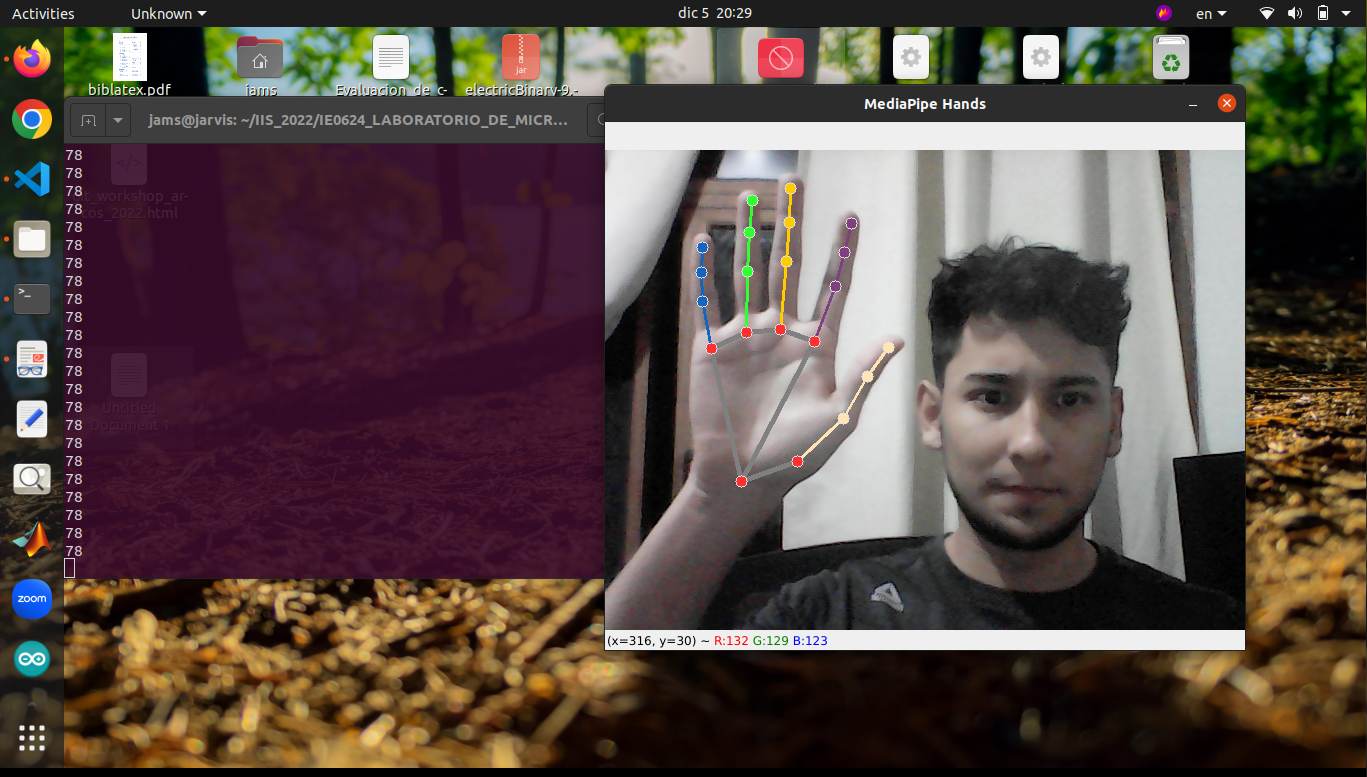
\includegraphics[scale=0.40]{./images/mano.png} 
\caption{Funcionalidad del script \texttt{hand\_recognizer.py} (Autoría propia).}
\label{mano}
\end{figure}

El funcionamiento de este script es acertado y no hay mucho más por analizar, pues su comprobación es simple. Registra aproximadamente 20 muestras por segundo y es un programa sólido.\\
Consiste primeramente en la integración de las librerías mencionadas anteriormente. Seguidamente se registran los parámetros deseados de la hora con en el orden \texttt{[hour, minute, second]} para posteriormente llegar al grueso del programa de visión por computador.\\
La sección que muestrea registra únicamente las coordenadas horizontales de la posición de la mano. En el entregable estas coordenadas no se imprimen, esto se implementa únicamente para verificar su funcionamiento. Seguidamente se entra a la parte de interacción serial con el arduino. Es muy importante resaltar que las muestras capturadas se envian como \texttt{string} al arduino por el anterior análsis dado en la sección del correspondiente al firmware. La comunicación serial presentó la dificultad de ser demasiada información para procesar por el arduino, pues el muestreo era mayor, con mayor cantidad de decimales, y con más precisión; dado esto, y debido a que para efectos de percepción humana en una señal analógica basta con al menos unos 10 puntos de luminosidad para cumplir con el objetivo del proyecto, se parametrizó las muestras en 10 estados. Los puntos de «posición» que tienen la capacidad de salir de la computadora hacia el arduino son 10: $[0, 10, 20, 30, 40, 50, 60, 70, 80, 90]$ La función \texttt{arduino} que es la encargada de enviar una parametrización de las muestras por el puerto serial, recibe un valor, dígase que este valor se encuentra entre 30 y 40, seguidamente ese valor se parametriza en en 30, y esta es la «señal» que se envía a través del puerto serial. Esto logró resolver el problema de las muestras excesivas y permitió evitar que el programa fuera más lento o se detuviera \textit{«crasheando»} la computadora.\\
Por último se crea la imagen que se ilustra en figura \ref{mano} para poder ver con facilidad los puntos específicos coloridos que registran la posición de la mano.